

The derivations for this benchmark are found in Section~\ref{ss:elastic_disc}.
we here recall the fields:
\begin{eqnarray}
\upnu_r          &=& \upnu_0 r^n \cos (k \theta)   \\
\upnu_\theta     &=& \upnu_0 r^n \sin (k \theta)   \\
\varepsilon_{rr} &=&   \upnu_0 n r^{n-1} \cos (k\theta) \\
\varepsilon_{\theta\theta} &=&    \upnu_0 r^{n-1} (k+1) \cos (k\theta) \\
\varepsilon_{r\theta} &=&  \cfrac{\upnu_0}{2}  r^{n-1}  (n-1-k)  \sin (k \theta)  \\
\end{eqnarray}


The disc has radius $R=1$. We set $\upnu_0$ and choose $\mu=1$, $\nu=0.25$ so that 
$\lambda=2\mu\nu/(1-2\nu)=1$.
The mesher is borrowed from \stone~58. The mesh consists of {\tt nLayers} concentric layers of elements.
We choose as 'diameter' of elements the value $h_r=R/nLayers$.



\begin{center}
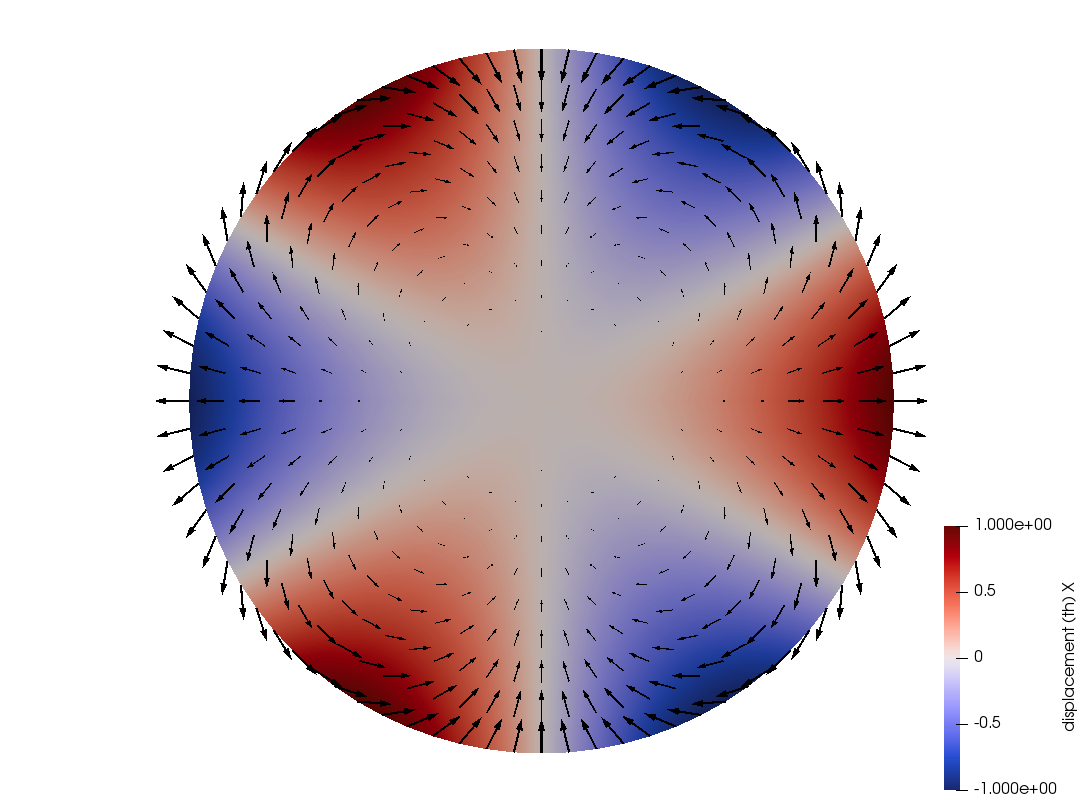
\includegraphics[width=5.7cm]{python_codes/fieldstone_111/u_k2}
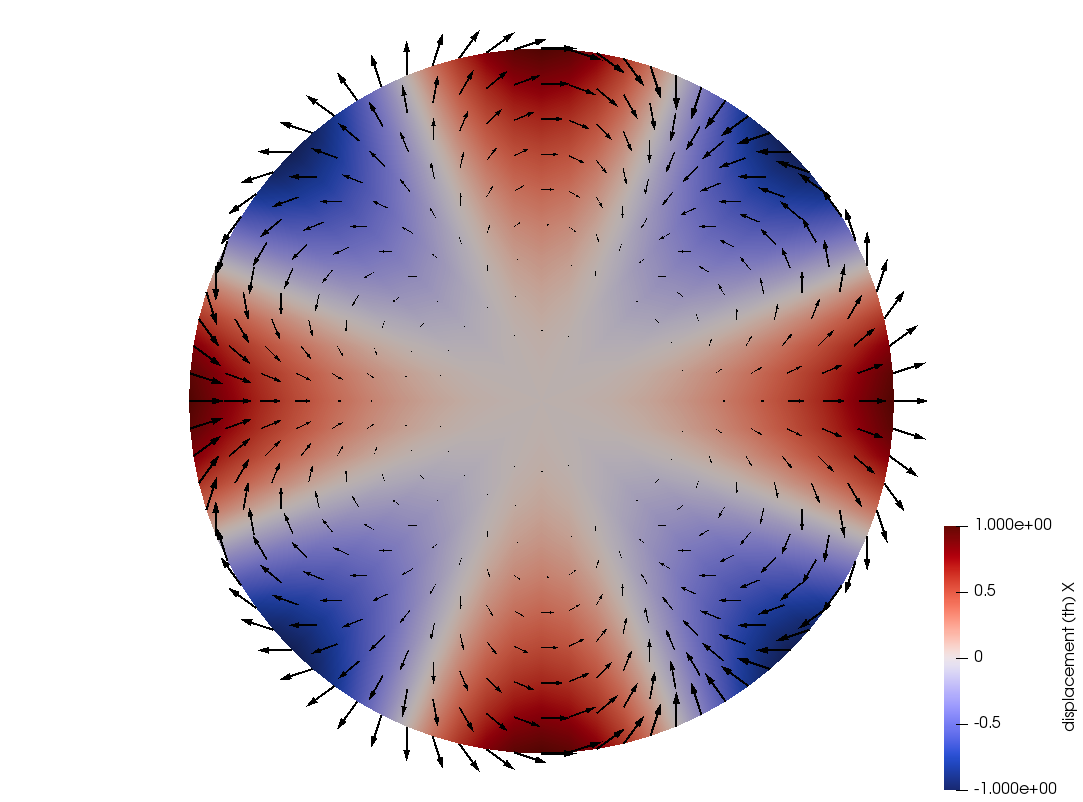
\includegraphics[width=5.7cm]{python_codes/fieldstone_111/u_k3}
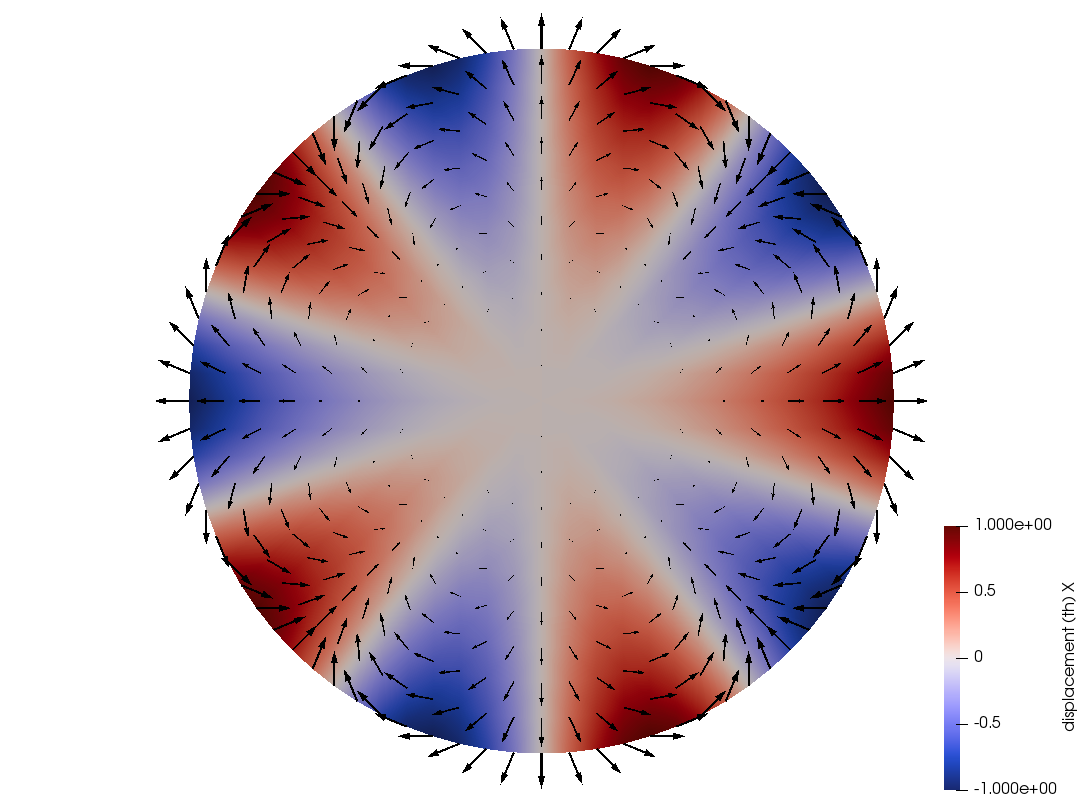
\includegraphics[width=5.7cm]{python_codes/fieldstone_111/u_k4}\\
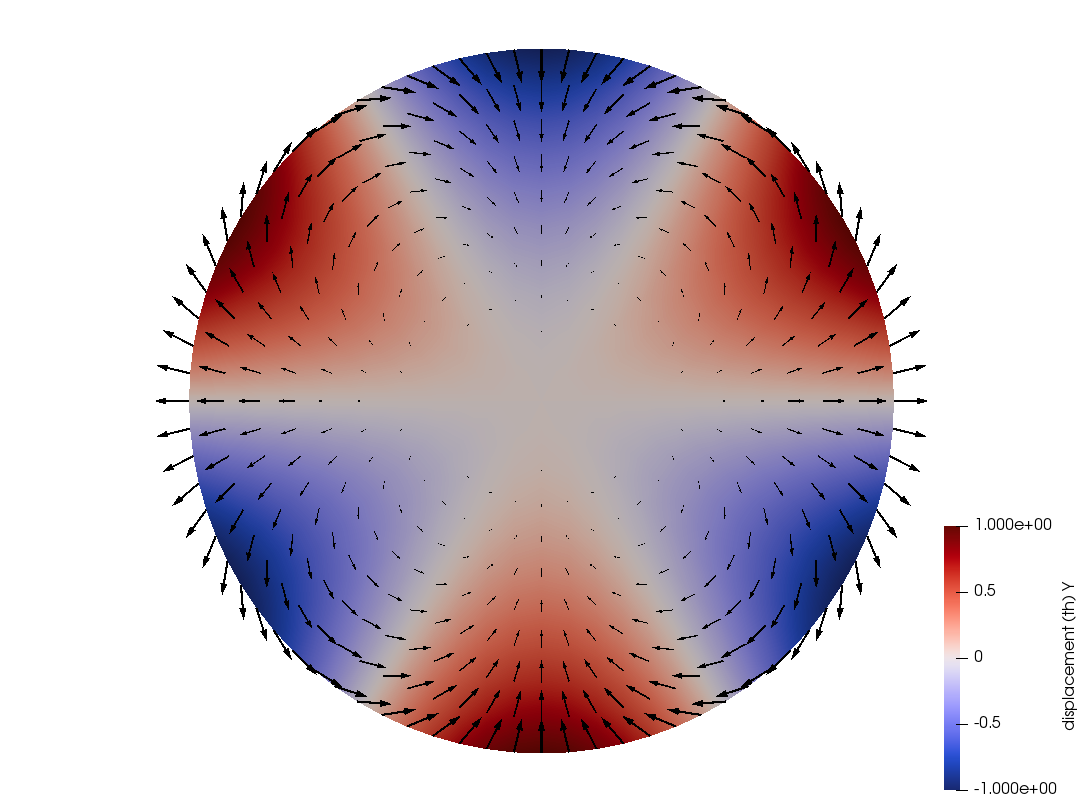
\includegraphics[width=5.7cm]{python_codes/fieldstone_111/v_k2}
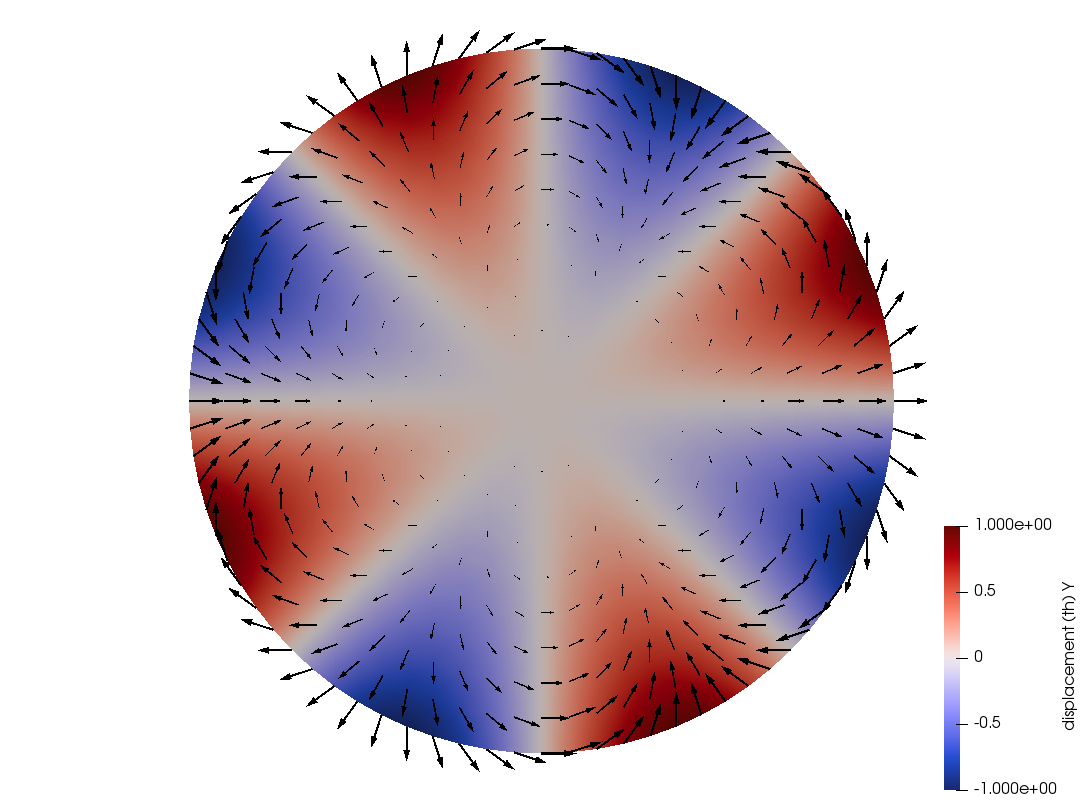
\includegraphics[width=5.7cm]{python_codes/fieldstone_111/v_k3}
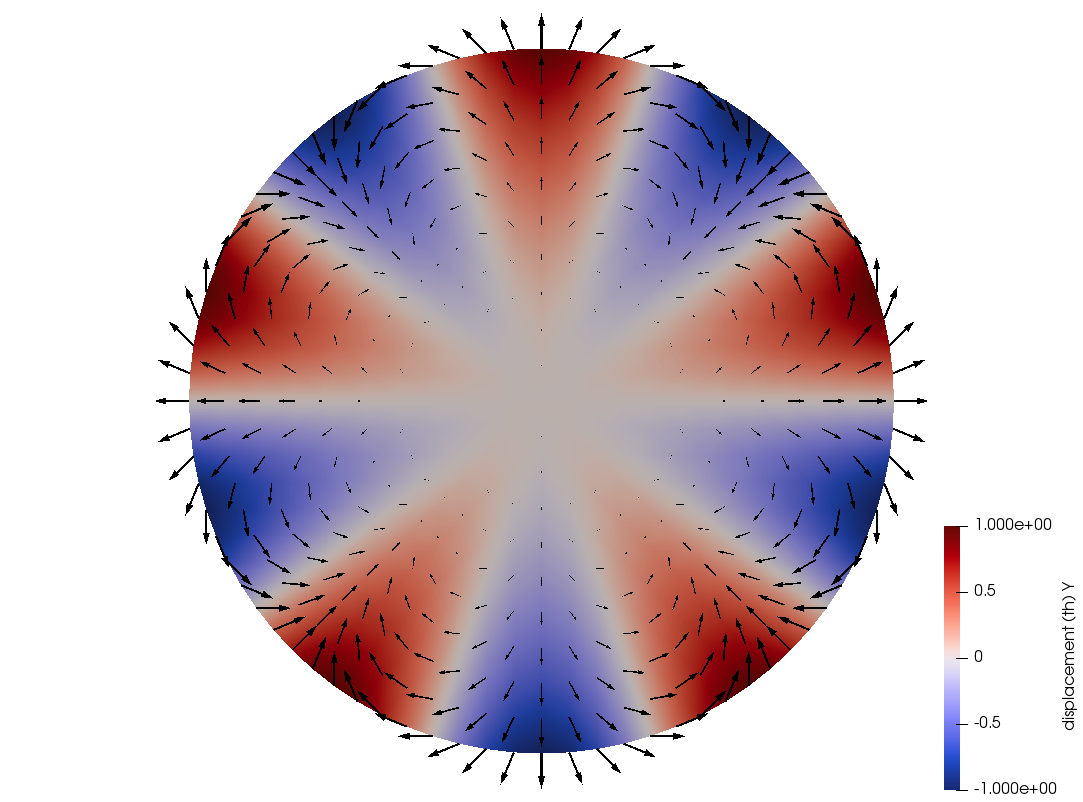
\includegraphics[width=5.7cm]{python_codes/fieldstone_111/v_k4}\\
{\captionfont Obtained for $n=2$. Left to right: $k=2,3,4$.}
\end{center}

